\documentclass[aspectratio=169]{beamer}
\mode<presentation> {
\usetheme{default}
\usecolortheme{dolphin}
}
\usepackage{algorithm,algorithmic}
\usepackage{caption}
\usepackage{multirow}
\usepackage{threeparttable}
\usepackage{graphicx}
\usepackage{parskip}
\usepackage{float}
\usepackage{alphabeta}
\usepackage{multirow,array}
\usepackage{subfig}
\usepackage{amsmath}
\usepackage{amssymb}
\usepackage{mathabx}
\usepackage{caption}
\usepackage{pifont} 
\usepackage{booktabs,tabularx}
\usepackage{tikz}
\usetikzlibrary{shapes,arrows}
\usepackage[table]{xcolor}
\newcolumntype{Y}{>{\raggedright\arraybackslash}X}

\usepackage{tikz}
\usetikzlibrary{arrows.meta,positioning,calc,fit,backgrounds,decorations.pathreplacing, shapes.geometric}
\graphicspath{{figures/}}
\usetikzlibrary{matrix,chains,positioning,decorations.pathreplacing,arrows}

% TikZ Styles - Adjusted font sizes for clarity since bold is removed
\tikzset{
  >=Stealth,
  st/.style={circle,draw,inner sep=0pt,minimum size=6mm, fill=white}, 
  action/.style={circle,fill=black,inner sep=0pt,minimum size=2mm},
  tr/.style={-Stealth, line width=0.8pt},
  lbl/.style={font=\footnotesize},
  block/.style={rectangle, draw, fill=blue!10, rounded corners, minimum height=2em}
}

\newcommand{\E}{\mathbb{E}}
\newcommand{\R}{\mathbb{R}}
\newcommand{\1}{\mathbf{1}}
\newcommand{\loss}{\mathcal{L}}
\newcommand{\X}{\mathcal{X}}
\newcommand{\Y}{\mathcal{Y}}
\newcommand{\D}{\mathcal{D}}
\newcommand{\thetavec}{\boldsymbol{\theta}}
\DeclareMathOperator*{\argmax}{arg\,max}
\DeclareMathOperator*{\argmin}{arg\,min}
\setbeamertemplate{caption}[numbered]
\setbeamertemplate{navigation symbols}{}
\setbeamertemplate{footline}[frame number]

\title{Lecture 10: Supervised Learning: Regression and Classification}

\author{Yasuyuki Sawada, Yaolang Zhong}
\institute{University of Tokyo\\
  \small \texttt{\href{mailto:yaolang.zhong@e.u-tokyo.ac.jp}{yaolang.zhong@e.u-tokyo.ac.jp}}}
\date{\today}

\begin{document}

\begin{frame}
\titlepage  
\end{frame}

% Slide 2: Lecture Overview
\begin{frame}{Lecture Overview}
    \begin{enumerate}
        \item Overview of Machine Learning
        \begin{itemize}
            \item The landscape: Supervised, Unsupervised, Reinforcement Learning
            \item A unified notation ($\mathcal{D}$, $f_\theta$, $\mathcal{L}$)
            \item The three-step optimization framework
        \end{itemize}
        
        \item Supervised Learning
        \begin{itemize}
            \item Regression: Linear models, Ridge \& Lasso regularization, the Bias-Variance trade-off
            \item Classification: Logistic regression, Confusion matrix,  the Precision-Recall trade-off
        \end{itemize}
        
        \item Training Neural Networks
        \begin{itemize}
            \item Automatic Differentiation (Backpropagation)
            \item Stochastic Gradient Descent
        \end{itemize}
    \end{enumerate}
\end{frame}


% -------------------------------------------------------------------------
% Section 2: Machine Learning Overview
% -------------------------------------------------------------------------
\section{Overview of Machine Learning}

% Slide 1: The Landscape (Taxonomy)
\begin{frame}{The Landscape of Machine Learning}
\small
    Machine Learning is the science of programming computers to learn from data.
    We generally categorize problems into three main paradigms based on the signal available to the learner:

    \vspace{0.5em}

    \begin{itemize}
        \setlength\itemsep{0.8em} % Increases space between main items
        
        \item 1. \textbf{Supervised Learning}: Learn to predict output $Y$ from input $X$.
        \begin{itemize}
            \item \textbf{Regression}: The output $Y$ is continuous (e.g., predicting house prices, temperature).
            \item \textbf{Classification}: The output $Y$ is categorical (e.g., spam detection, image recognition).
        \end{itemize}

        \item 2. \textbf{Unsupervised Learning}: Discover structure within input $X$ (no labels $Y$).
        \begin{itemize}
            \item Clustering: Grouping similar data points together.
            \item Dimensionality Reduction: Compressing data while preserving information.
        \end{itemize}

        \item 3. \textbf{Reinforcement Learning}: Learn a policy to maximize rewards via interaction.
        \begin{itemize}
            \item Agent-Environment Loop: The learner performs actions which affect future states.
            \item Feedback: Learning relies on delayed reward signals rather than immediate correct answers.
        \end{itemize}
    \end{itemize}
\end{frame}

% Slide 2: The Unified Notation
\begin{frame}{A Unified Notation for All Tasks}
    
    
    Despite their differences, all three tasks share the same mathematical skeleton.
    
    \begin{block}{The Universal Components}
    \begin{enumerate}
        \item \textbf{The Data} ($\D$): 
        \begin{itemize}
            \item Supervised: Pairs of $\{(x_i, y_i)\}$.
            \item Unsupervised: Just features $\{x_i\}$.
            \item RL: Trajectories of $\{(s_t, a_t, r_{t+1}, s_{t+1})\}$.
        \end{itemize}
        
        \item \textbf{The Model} ($f_{\theta}$): 
        The function we wish to learn, parameterized by $\theta$.
        $$ \hat{y} = f_\theta(x) \quad \text{or} \quad \pi_\theta(a|s) $$
        
        \item \textbf{The Objective} ($\loss$): 
        A Loss (or Reward) function measuring performance.
        $$ \min_{\theta} \mathcal{L}(f_\theta(\D)) $$
    \end{enumerate}
    \end{block}
\end{frame}




\begin{frame}{The Three-Step Optimization Framework}
    \small
    \vspace{0.3mm}

    \begin{itemize}
        \item Step 1 (Data $\D$): Collect or sample the training data.
        \begin{itemize}
            \item Supervised: pairs $\{(x_i, y_i)\}_{i=1}^M$ drawn from true distribution.
            \item The quality and quantity of $\D$ fundamentally bounds what we can learn.
        \end{itemize}
        
        \item Step 2 (Model $f_\theta$): Choose a parameterized function class.
        \begin{itemize}
            \item Linear: $f_\theta(x) = \theta^\top x$. \quad Neural Network: $f_\theta(x) = \sigma(W_L \cdots \sigma(W_1 x))$.
            \item The architecture determines the \textit{hypothesis space} we search over.
        \end{itemize}

        \item Step 3 (Objective $\loss$ + Solver): Define loss and optimize.
        \begin{itemize}
            \item Loss function $\ell$: The function that measures how far the model's predictions are from the true values.
            \item Define objective: $\displaystyle \min_{\theta} \loss(\theta) = \frac{1}{M} \sum_{i=1}^M \ell\big(f_\theta(x_i), y_i\big)$
            \item Solve via Gradient Descent: $\theta_{t+1} = \theta_t - \alpha \nabla_\theta \loss(\theta)$
        \end{itemize}
    \end{itemize}
    \end{frame}





% -------------------------------------------------------------------------
% Section 3: Supervised Learning
% -------------------------------------------------------------------------
\section{Supervised Learning}

% Slide 1: Overview - Prediction vs Inference
\begin{frame}{Supervised Learning: Prediction vs. Inference}
    \small
    \vspace{0.5em}
    The Setup: Given data $\D$, we estimate $f$ such that $Y \approx f(X)$.
    The \textit{objective} dictates the methodology:
    \begin{itemize}
        \setlength\itemsep{1.2em} 
        
        \item \textbf{1. Prediction (Focus on $\hat{Y}$)}
        \begin{itemize}
            \item Goal: Minimize error on new inputs (Accuracy is king).
            \item Trade-off: We accept complex "Black Box" models if they predict well.
            \item Typical Use: Pattern recognition, Forecasting, Churn prediction.
        \end{itemize}

        \item \textbf{2. Inference (Focus on $\hat{f}$ and $\hat{\theta}$)}
        \begin{itemize}
            \item Goal: Interpret the \textit{mechanism}. We need the functional form and parameter significance (e.g., Elasticity).
            \item The Causal Challenge: 
            Inference often implies seeking \textit{Causality}. However, standard ML optimizes for \textit{Correlation}, not Identification.
            \item Crucial Caveat: 
            Standard ML does not solve the Endogeneity Problem ($X \perp \epsilon$ is assumed). Identification strategies are required for causal claims but are beyond today's scope.
        \end{itemize}
    \end{itemize}
\end{frame}

% Slide 2: Regression Definitions
\begin{frame}{Task 1: Regression (Definitions)}
    Definition:
    Regression covers problems where the response variable $Y$ is quantitative (numerical, continuous). Examples: Salary, Blood Pressure, House Price.

    \vspace{0.5em}
    The Model:
    We assume the true relationship is:
    $$ Y = f(X) + \epsilon $$
    where $f(X)$ is the systematic information provided by $X$, and $\epsilon$ is an irreducible error term (mean zero).

    \vspace{0.5em}
    The Loss Function (Mean Squared Error):
    To train the model (estimate $\hat{f}$), we minimize the average squared difference:
    $$ \text{MSE} = \frac{1}{n} \sum_{i=1}^n \left( y_i - \hat{f}(x_i) \right)^2 $$
\end{frame}

% Slide 3: Regression Example (Added)
\begin{frame}{Task 1: Regression (Example \& Functional Form)}
    Problem: Predict \textit{House Price} ($Y$) based on \textit{Square Footage} ($X_1$) and \textit{Number of Bedrooms} ($X_2$).
    
    \vspace{1em}
    Functional Form: Linear Regression
    The simplest form for $f(X)$ is a linear combination of inputs:
    $$ f(X) = \beta_0 + \beta_1 X_1 + \beta_2 X_2 $$
    
    \begin{itemize}
        \item Parameters ($\theta$): The coefficients $\beta = (\beta_0, \beta_1, \beta_2)$.
        \item Interpretation: $\beta_1$ represents the average increase in Price for one additional unit of Square Footage, holding Bedrooms constant.
        \item Learning: We find the specific $\beta$ values that minimize the Residual Sum of Squares (RSS).
    \end{itemize}
\end{frame}


% Slide 4: Motivation for Regularization
\begin{frame}{Regression with Many Covariates: Motivation}
    Problem:
    When the number of covariates is large or regressors are highly correlated:
    \begin{itemize}
        \item Ordinary Least Squares (OLS) estimates can have high variance.
        \item The model may overfit the training data.
        \item Interpretation becomes unstable due to multicollinearity.
    \end{itemize}

    \vspace{0.8em}
    Solution: Regularization

    We modify the regression objective by adding a penalty term that discourages large coefficients:
    \[
    \text{Loss} = \text{Fit to data} + \text{Penalty on model complexity}.
    \]

    This improves out-of-sample prediction by trading off bias and variance.
\end{frame}

% Slide 5: Ridge and Lasso Regression
\begin{frame}{Regularized Regression: Ridge and Lasso}
    \small
    Consider the linear model: $y_i = \beta_0 + X_i'\beta + \varepsilon_i$.

    \vspace{0.4em}
    \textbf{Ridge Regression} (L2 penalty):
    \vspace{-0.3em}
    \[
    \min_{\beta} \;
    \frac{1}{n} \sum_{i=1}^n (y_i - X_i'\beta)^2
    \;+\;
    \lambda \sum_{j=1}^p \beta_j^2
    \]
    \vspace{-0.5em}
    Shrinks coefficients toward zero; reduces variance, keeps all covariates.

    \vspace{0.3em}
    \textbf{Lasso Regression} (L1 penalty):
    \vspace{-0.3em}
    \[
    \min_{\beta} \;
    \frac{1}{n} \sum_{i=1}^n (y_i - X_i'\beta)^2
    \;+\;
    \lambda \sum_{j=1}^p |\beta_j|
    \]
    \vspace{-0.5em}
    Performs shrinkage and variable selection; some coefficients set exactly to zero.
\end{frame}


% Slide 6: Intuition Behind Ridge and Lasso (Geometric View)
\begin{frame}{Intuition: How Ridge and Lasso Shrink Coefficients}
    \small
    Consider the constrained form of the optimization:

    \vspace{0.3em}
    Ridge (L2): $\min_{\beta} \text{RSS}(\beta)$ s.t. $\sum_{j} \beta_j^2 \leq c$
    \quad
    Lasso (L1): $\min_{\beta} \text{RSS}(\beta)$ s.t. $\sum_{j} |\beta_j| \leq c$

    \vspace{0.4em}
    Key intuition:
    \begin{itemize}
        \setlength\itemsep{0.2em}
        \item RSS has elliptical level sets centered at OLS solution.
        \item Ridge: circular constraint $\Rightarrow$ smooth shrinkage.
        \item Lasso: diamond constraint $\Rightarrow$ coefficients hit corners (sparse).
    \end{itemize}
\end{frame}


% Slide: Shrinkage Geometry
\begin{frame}{Shrinkage Intuition: Ridge vs Lasso}

    \begin{center}
    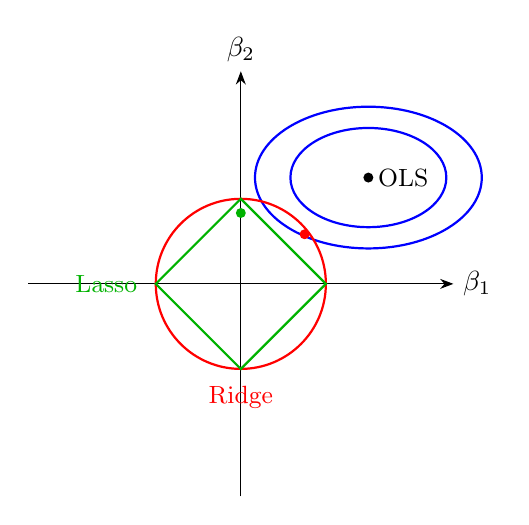
\begin{tikzpicture}[scale=0.9]
    
    % Axes
    \draw[->] (-3,0) -- (3,0) node[right] {$\beta_1$};
    \draw[->] (0,-3) -- (0,3) node[above] {$\beta_2$};
    
    % OLS point
    \fill (1.8,1.5) circle (2pt);
    \node[right] at (1.8,1.5) {\small OLS};
    
    % RSS contours
    \draw[blue, thick] (1.8,1.5) ellipse (1.6 and 1.0);
    \draw[blue, thick] (1.8,1.5) ellipse (1.1 and 0.7);
    
    % Ridge constraint (circle)
    \draw[red, thick] (0,0) circle (1.2);
    \node[red] at (0,-1.6) {\small Ridge};
    
    % Lasso constraint (diamond)
    \draw[green!70!black, thick]
      (1.2,0) -- (0,1.2) -- (-1.2,0) -- (0,-1.2) -- cycle;
    \node[green!70!black] at (-1.9,0) {\small Lasso};
    
    % Ridge solution
    \fill[red] (0.9,0.7) circle (2pt);
    
    % Lasso solution (on axis)
    \fill[green!70!black] (0,1.0) circle (2pt);
    
    \end{tikzpicture}
    \end{center}
    
    \vspace{0.5em}
    \begin{itemize}
        \item Ridge shrinks coefficients smoothly toward zero.
        \item Lasso often sets coefficients exactly equal to zero.
    \end{itemize}
    
    \end{frame}


\begin{frame}{The Bias-Variance Trade-off}
    \small
    One of the most important concepts in Supervised Learning (ISLP 2.2.2).
    It explains why we don't simply use the most complex model possible to fit the training data perfectly.

    Decomposition of Expected Test Error:
    For a test point $x_0$ where $y_0 = f(x_0) + \epsilon$ with $E[\epsilon]=0$, $\text{Var}(\epsilon)=\sigma^2$:
    \begin{align*}
    E\left[ (y_0 - \hat{f}(x_0))^2 \right] &= E\left[ (f(x_0) + \epsilon - \hat{f}(x_0))^2 \right] \\[0.3em]
    &= \underbrace{E\left[(\hat{f}(x_0) - E[\hat{f}(x_0)])^2\right]}_{\text{Variance of } \hat{f}} + \underbrace{(E[\hat{f}(x_0)] - f(x_0))^2}_{\text{Bias}^2} + \underbrace{\sigma^2}_{\text{Noise}}
    \end{align*}

    \begin{itemize}
        \item \textbf{Variance}: Sensitivity to the training set. (High complexity $\to$ High Variance $\to$ Overfitting).
        \item \textbf{Bias}: Error from simplifying assumptions. (Low complexity $\to$ High Bias $\to$ Underfitting).
        \item \textbf{Irreducible Error}: The noise floor inherent in the data.
    \end{itemize}

    The Challenge:
    As we increase model complexity, Bias $\downarrow$ but Variance $\uparrow$. We must find the "sweet spot" (U-shaped curve) that minimizes the \textit{sum} of both.
\end{frame}

    

% Slide 4: Classification Definitions
\begin{frame}{Task 2: Classification (Definitions)}
    Definition:
    Classification covers problems where the response $Y$ is qualitative (categorical).
    The values of $Y$ belong to a finite set of classes $\mathcal{C}$ (e.g., $\{\text{Spam, Ham}\}$ or $\{\text{Cat, Dog, Fox}\}$).

    \vspace{0.5em}
    The Goal:
    We build a classifier $C(X)$ to assign a class label to a new observation.
    Often, we first estimate the conditional probability:
    $$ \hat{p}_k(x) = \Pr(Y = k \mid X = x) $$
    We then classify to the class with the highest probability (Bayes Classifier).

    \vspace{0.5em}
    The Loss Function (Error Rate):
    We minimize the fraction of misclassifications: $\frac{1}{n} \sum I(y_i \neq \hat{y}_i)$.
\end{frame}

% Slide 5: Classification Example (Added)
\begin{frame}{Task 2: Classification (Example \& Functional Form)}
    Problem: Predict \textit{Default Status} ($Y \in \{0, 1\}$) based on \textit{Credit Balance} ($X$).
    
    
    \vspace{1em}
    Functional Form: Logistic Regression
    We cannot use a straight line because probabilities must be between 0 and 1. Instead, we use the Logistic Function (Sigmoid):
    
    $$ p(X) = \frac{e^{\beta_0 + \beta_1 X}}{1 + e^{\beta_0 + \beta_1 X}} $$
    
    \begin{itemize}
        \item Mechanism: This S-shaped curve squashes any input value into the range $[0, 1]$.
        \item Decision Boundary: If $p(X) > 0.5$, we predict "Default" (1); otherwise "No Default" (0).
        \item Learning: We find $\beta$ by maximizing the Likelihood of the observed data.
    \end{itemize}
\end{frame}

% Slide: Confusion Matrix
\begin{frame}{Classification Metrics: The Confusion Matrix}
    \small
    Why Accuracy Isn't Enough:
    In binary classification (e.g., disease detection), a naive model predicting ``No Disease'' for everyone achieves 99\% accuracy if only 1\% are sick—but it's useless.

    \vspace{0.1em}
    The Confusion Matrix breaks down predictions into four outcomes:
    
    \vspace{0.1em}
    \begin{center}
    \renewcommand{\arraystretch}{1.2}
    \begin{tabular}{|c|c|c|}
        \hline
         & Actual Positive (1) & Actual Negative (0) \\ \hline
        Predicted Positive 
        & \cellcolor{green!25} True Positive (TP) 
        & \cellcolor{red!25} False Positive (FP) \\ \hline
        Predicted Negative 
        & \cellcolor{orange!25} False Negative (FN) 
        & True Negative (TN) \\ \hline
    \end{tabular}
    \end{center}
    
    \vspace{0.2em}
    \begin{itemize}
        \setlength\itemsep{0.1em}
        \item \textbf{TP}: Correctly identified positives. \textbf{TN}: Correctly identified negatives.
        \item \textbf{FP} (Type I): False alarm. \textbf{FN} (Type II): Missed positive.
        \item \textbf{Precision} $=$ \textcolor{green!70!black}{TP}$/($\textcolor{green!70!black}{TP}$+$\textcolor{red!70!black}{FP}$)$ — of predicted positives, how many correct?
        \item \textbf{Recall} $=$ \textcolor{green!70!black}{TP}$/($\textcolor{green!70!black}{TP}$+$\textcolor{orange!70!black}{FN}$)$ — of actual positives, how many detected?
    \end{itemize}
\end{frame}

% Slide: The Precision--Recall Trade-off
\begin{frame}{The Precision--Recall Trade-off}
    \small
    Key idea:  
    Changing the decision threshold $\tau$ trades off Precision and Recall.
    
    \begin{itemize}
        \setlength\itemsep{0.3em}
        \item Lower threshold (predict positives more easily):
        Recall $\uparrow$, Precision $\downarrow$
    
        \item Higher threshold (predict positives more cautiously):
        Precision $\uparrow$, Recall $\downarrow$
    \end{itemize}
    
    \vspace{0.4em}
    Why this is different from regression:
    \begin{itemize}
        \setlength\itemsep{0.2em}
        \item Regression uses a single metric (e.g., MSE).
        \item Classification needs multiple metrics because:
        \begin{itemize}
            \item classes may be imbalanced,
            \item FP and FN have different costs,
            \item the optimal threshold depends on the application.
        \end{itemize}
    \end{itemize}
\end{frame}


\begin{frame}{Training Neural Networks: Automatic Differentiation}
    \small
    \begin{itemize}
        \setlength\itemsep{0.4em}
        \item A neural network is a composition of functions: $\hat{y} = f(x; \theta)$, where $\theta$ collects weights and biases.
    
        \item To train, we need gradients $\nabla_\theta \mathcal{L}$. Manual differentiation is impractical for deep networks.
    
        \item \textbf{Automatic Differentiation} (Auto-diff):
        \begin{itemize}
            \item Libraries (PyTorch, TensorFlow) record operations during the forward pass.
            \item These form a \textbf{computational graph}; chain rule applied in reverse (\textbf{backpropagation}).
        \end{itemize}
    
        \item Key takeaway: Auto-diff gives \textbf{exact gradients} with cost $\approx$ one forward pass.
    \end{itemize}
\end{frame}


% Slide: Automatic Differentiation
\begin{frame}{Training Neural Networks: Automatic Differentiation}
\small

\begin{columns}
\column{0.55\textwidth}
\begin{itemize}
    \item Neural networks are built from many simple operations.
    \item During the forward pass, each operation is recorded.
    \item These operations form a computational graph.
    \item Auto-diff applies the chain rule automatically backward.
\end{itemize}

\vspace{0.6em}
Key idea:  
Gradients are computed exactly, without manual differentiation.

\column{0.45\textwidth}

\begin{center}
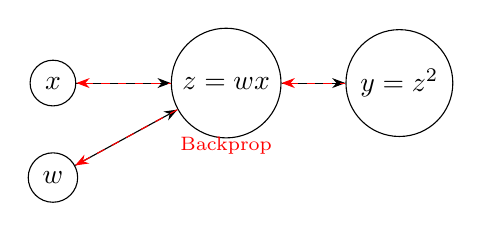
\begin{tikzpicture}[node distance=1.2cm]

\node (x) [draw, circle] {$x$};
\node (w) [draw, circle, below of=x] {$w$};
\node (z) [draw, circle, right of=x, xshift=1cm] {$z = wx$};
\node (y) [draw, circle, right of=z, xshift=1cm] {$y = z^2$};

\draw[->] (x) -- (z);
\draw[->] (w) -- (z);
\draw[->] (z) -- (y);

\draw[<- , dashed, red] (z) -- (y);
\draw[<- , dashed, red] (x) -- (z);
\draw[<- , dashed, red] (w) -- (z);

\node[red, below of=z, yshift=0.4cm] {\scriptsize Backprop};

\end{tikzpicture}
\end{center}

\end{columns}
\end{frame}

\begin{frame}{Training Neural Networks: Stochastic Gradient Descent}
    \small
    Objective: Minimize average loss: $\mathcal{L}(\theta) = \frac{1}{M} \sum_{i=1}^M \ell_i(\theta)$
    
    \vspace{0.3em}
    \begin{itemize}
        \setlength\itemsep{0.3em}
        \item \textbf{Full Gradient Descent}: Computes gradients using all $M$ observations. Accurate but expensive when $M$ is large.
    
        \item \textbf{Stochastic (Mini-Batch) GD}:
        \begin{itemize}
            \item Sample a small batch; form a noisy but cheap gradient estimate.
            \item Update: $\theta \leftarrow \theta - \alpha \, \nabla_\theta \mathcal{L}_{\text{batch}}$
        \end{itemize}
    
        \item Why it works: Each update is fast; noise aids exploration; many small steps approximate full GD.
    \end{itemize}
\end{frame}

% Slide: Stochastic Gradient Descent
\begin{frame}{Training Neural Networks: Stochastic Gradient Descent}
    \small
    
    \begin{columns}
    \column{0.55\textwidth}
    \begin{itemize}
        \item Goal: minimize average loss over a large dataset.
        \item Full gradient descent:
        \begin{itemize}
            \item Uses all data each step
            \item Accurate but slow
        \end{itemize}
        \item Stochastic gradient descent (SGD):
        \begin{itemize}
            \item Uses small random batches
            \item Fast but noisy updates
        \end{itemize}
    \end{itemize}
    
    \vspace{0.5em}
    Key idea:  
    Many cheap noisy steps can outperform a few expensive exact steps.
    
    \column{0.45\textwidth}
    
    \begin{center}
    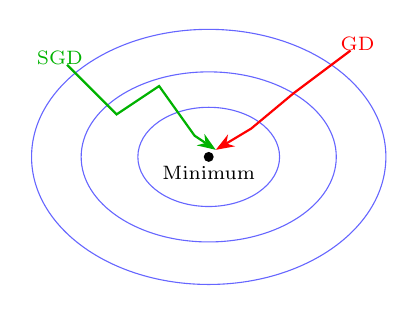
\begin{tikzpicture}[scale=0.9]
    
    % Loss contours
    \draw[blue!60] (0,0) ellipse (2.5 and 1.8);
    \draw[blue!60] (0,0) ellipse (1.8 and 1.2);
    \draw[blue!60] (0,0) ellipse (1.0 and 0.7);
    
    % Minimum
    \fill (0,0) circle (2pt);
    \node[below] at (0,0) {\scriptsize Minimum};
    
    % Full GD path
    \draw[red, thick, ->] (2,1.5) -- (1.2,0.9) -- (0.6,0.4) -- (0.1,0.1);
    \node[red] at (2.1,1.6) {\scriptsize GD};
    
    % SGD path
    \draw[green!70!black, thick, ->]
        (-2,1.3) -- (-1.3,0.6) -- (-0.7,1.0) -- (-0.2,0.3) -- (0.1,0.1);
    \node[green!70!black] at (-2.1,1.4) {\scriptsize SGD};
    
    \end{tikzpicture}
    \end{center}
    
    \end{columns}
    \end{frame}
% -------------------------------------------------------------------------
% Section 4: Unsupervised Learning
% -------------------------------------------------------------------------
% \section{Unsupervised Learning}

% % Slide 1: Overview
% \begin{frame}{Unsupervised Learning: Overview}
%     The Setup (ISLP Ch 12):
%     We observe input vectors $X_1, \dots, X_n$, but we have no associated response $Y$.
%     $$ \D = \{x_1, x_2, \dots, x_n\} $$
    
%     The Challenge:
%     Without a target $Y$ to predict, we cannot calculate a simple "error" (like MSE). There is no "teacher" to correct the model.
    
%     The Goal:
%     We seek to discover interesting things about the measurements:
%     \begin{itemize}
%         \item Is there an informative way to visualize the data?
%         \item Can we discover subgroups among the variables or observations?
%         \item Can we describe the underlying distribution $P(X)$?
%     \end{itemize}
% \end{frame}

% % Slide 2: Clustering Definitions
% \begin{frame}{Task 1: Clustering (Definitions)}
%     Definition:
%     Clustering refers to a broad set of techniques for finding \textit{subgroups}, or \textit{clusters}, in a dataset.
    
%     The Goal:
%     Partition the data into distinct groups such that:
%     \begin{itemize}
%         \item Observations within each group are quite similar to each other.
%         \item Observations in different groups are quite different from each other.
%     \end{itemize}
    
%     The Logic:
%     We must define a metric for "similarity" (usually Euclidean distance). The algorithm then searches for the grouping that maximizes this similarity.
% \end{frame}

% % Slide 3: Clustering Example
% \begin{frame}{Task 1: Clustering (Example \& Mechanism)}
%     Problem: \textit{Market Segmentation}.
%     Given spending history ($X$) of thousands of customers, identify distinct "personas" (e.g., "Budget Shoppers" vs. "High Spenders").
    
%     \centering
    
    
%     \vspace{0.5em}
%     \raggedright
%     Mechanism: K-Means Clustering
%     We want to partition observations into $K$ sets. We solve this by minimizing the Within-Cluster Variation:
    
%     $$ \min_{C_1, \dots, C_K} \sum_{k=1}^K \sum_{i \in C_k} || x_i - \mu_k ||^2 $$
    
%     \begin{itemize}
%         \item $\mu_k$ is the center (centroid) of cluster $k$.
%         \item The algorithm iteratively assigns points to the nearest centroid, then updates the centroids to the mean of the assigned points.
%     \end{itemize}
% \end{frame}

% % Slide 4: Dimensionality Reduction Definitions
% \begin{frame}{Task 2: Dimensionality Reduction (Definitions)}
%     Definition:
%     Dimensionality Reduction reduces the number of random variables under consideration by obtaining a set of "principal" variables.
    
%     The Motivation:
%     \begin{itemize}
%         \item Visualization: We cannot visualize data in 100 dimensions. We need to project it down to 2 or 3.
%         \item Noise Reduction: Ignore small fluctuations and focus on the main trends.
%         \item Preprocessing: Make subsequent Supervised Learning tasks easier (avoiding the "Curse of Dimensionality").
%     \end{itemize}
% \end{frame}

% % Slide 5: Dimensionality Reduction Example
% \begin{frame}{Task 2: Dimensionality Reduction (Example \& Mechanism)}
%     Problem: \textit{Visualizing Genetic Data}.
%     We have gene expression levels for $p=10,000$ genes across $n=50$ patients. We want to see if patients group naturally.
    
%     \centering
    
    
%     \vspace{0.5em}
%     \raggedright
%     Mechanism: Principal Component Analysis (PCA)
%     We construct new variables $Z_1, Z_2, \dots$ that are linear combinations of the original features $X$:
%     $$ Z_1 = \phi_{11}X_1 + \phi_{21}X_2 + \dots + \phi_{p1}X_p $$
    
%     \begin{itemize}
%         \item Objective: Find the combination weights $\phi$ such that $Z_1$ captures the maximum possible variance in the data.
%         \item $Z_2$ is found next, maximizing remaining variance (uncorrelated to $Z_1$).
%         \item We typically keep only the first few components ($Z_1, Z_2$).
%     \end{itemize}
% \end{frame}


\begin{frame}{References}
    \begin{thebibliography}{10}
        
        \bibitem{hastie}
        James, G., Witten, D., Hastie, T., Tibshirani, R. (2021).
        \newblock \textit{An Introduction to Statistical Learning with Applications in Python}.
        \newblock Springer.
        \newblock \url{https://www.statlearning.com/}
        
        \bibitem{recap}
        Previous Lecture Notes.
        \newblock \textit{Optimization Frameworks for Neural Networks}.
        
    \end{thebibliography}
\end{frame}

\end{document}